\documentclass{article}
\usepackage{CJK}
\usepackage{ctex}
\usepackage{graphicx}
\usepackage{float}
\usepackage[colorlinks,linkcolor=black]{hyperref}
\graphicspath{{pic/}}
\renewcommand{\contentsname}{目录}
\renewcommand{\abstractname}{摘要}
\title{MusiCube - 手势音游\\
       项目期末报告}
\author{杨铭 - 5130379022\\
        李晟 - 5130379017\\
        张云翔 - 5130379012}
\begin{document}
\maketitle
\tableofcontents
\newpage
\section{项目概述}
\paragraph{}
电子游戏,被认为是第九大艺术,在电子产品和网络愈发普及的今天,被越来越多的人所承认和喜爱。而作为游戏中一种独特的类型——音乐游戏(MUG),由最早的街机发展而来,因其与音乐的结合,受到不少玩家的喜爱。
\paragraph{}
而随着VR,AR等概念的兴起,电子游戏的玩法也将出现新的变革。MusiCube就是一款突破性的音乐游戏,它使用了不同于之前音乐游戏键盘,鼠标或是手台的输入方式,利用LeapMotion的手势识别,让玩家可以更加自由地感受音乐游戏的快感。
\paragraph{}
在MusiCube中,所用的音符节拍将都在一个立体的魔方上出现,玩家可以通过手部的动作来操作魔方表面的音符,如戳击一个块,旋转一层。不仅如此,我们还提供图谱编辑器,玩家可以自由编辑自己的图谱,将来如果可能,还可以建立玩家社区,集排名,作
图,讨论,自定义皮肤等功能于一体,丰富游戏的玩法,提升游戏的深度,增加玩家的粘性。
\begin{figure}[H]
  % Requires \usepackage{graphicx}
  \begin{minipage}{0.5\linewidth}
    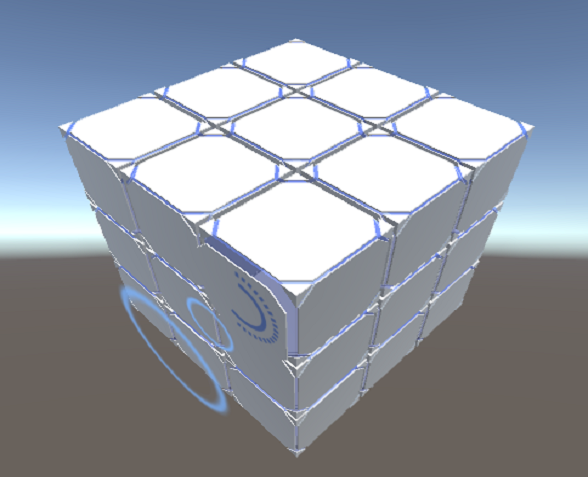
\includegraphics[width=15em]{mid-demo1.png}\\
    \caption{}\label{demo1}
  \end{minipage}
  \begin{minipage}{0.5\linewidth}
    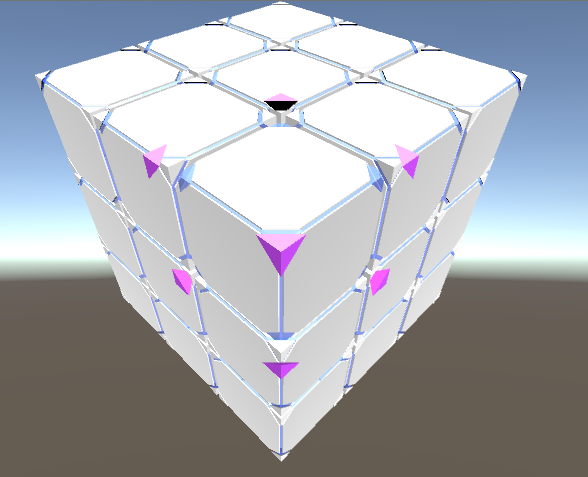
\includegraphics[width=15em]{mid-demo2.png}\\
    \caption{}\label{demo2}
  \end{minipage}
\end{figure}
\begin{description}
  \item[软件类型] 游戏 - 音乐游戏(MUG)
  \item[目标用户] PC用户、游戏玩家
  \item[平台支持] PC - Windows7及以上版本
  \item[硬件支持] LeapMotion
\end{description}
\newpage
\section{软件设计}
\subsection{架构设计}
本软件主要采用Unity3D制作,通过LeapMotion或者键盘鼠标来进行用户交互。软件进
入主界面后,可以选择进入选歌游玩界面或者选歌编辑界面。
\begin{figure}[H]
  \centering
  % Requires \usepackage{graphicx}
  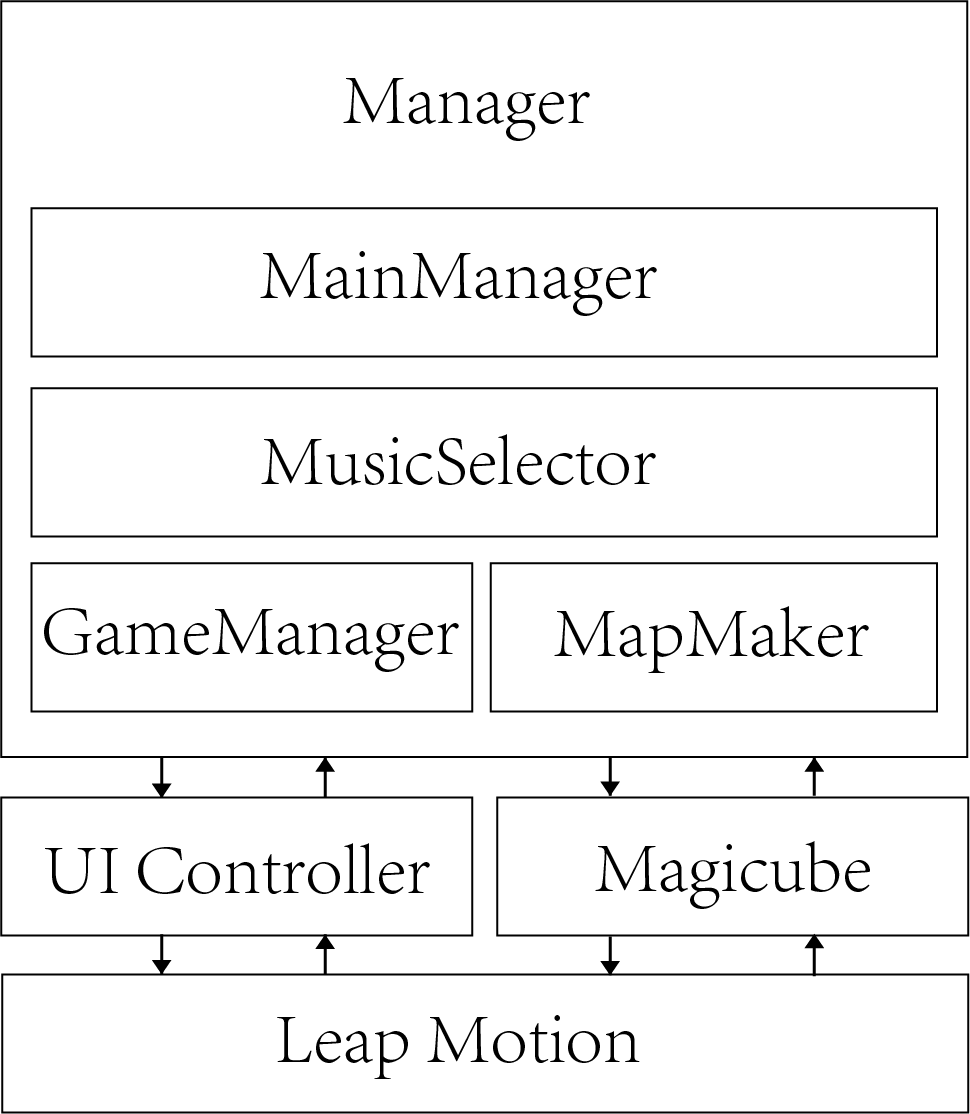
\includegraphics[width=20em]{arc-new.png}\\
  \caption{}\label{}
\end{figure}
\begin{description}
  \item[MainManager] 场景管理类,负责管理主菜单和各个场景见的切换
  \item[MusicSelector] 选歌界面的管理类,包括两个实力,分别管理选歌游玩和
      选歌编辑
  \item[MapMaker] 包含一个Magicube,为编辑图谱提供许多接口,并可以根据BPM
      (每分钟节拍数)划分时间轴和制作图谱
  \item[GameManager] 游戏管理类,负责接收Magicube传来的Note数据并进行判定
  \item[UI Controller] 在各个场景都有,负责用户和UI的交互
  \item[Magicube] 游戏主题魔方的主题,管理27个方块负责播放游戏动画和音乐
  \item[LeapMotion] 用户进行输入的设备
\end{description}
\textbf{流程图}
\begin{figure}[H]
  \centering
  % Requires \usepackage{graphicx}
  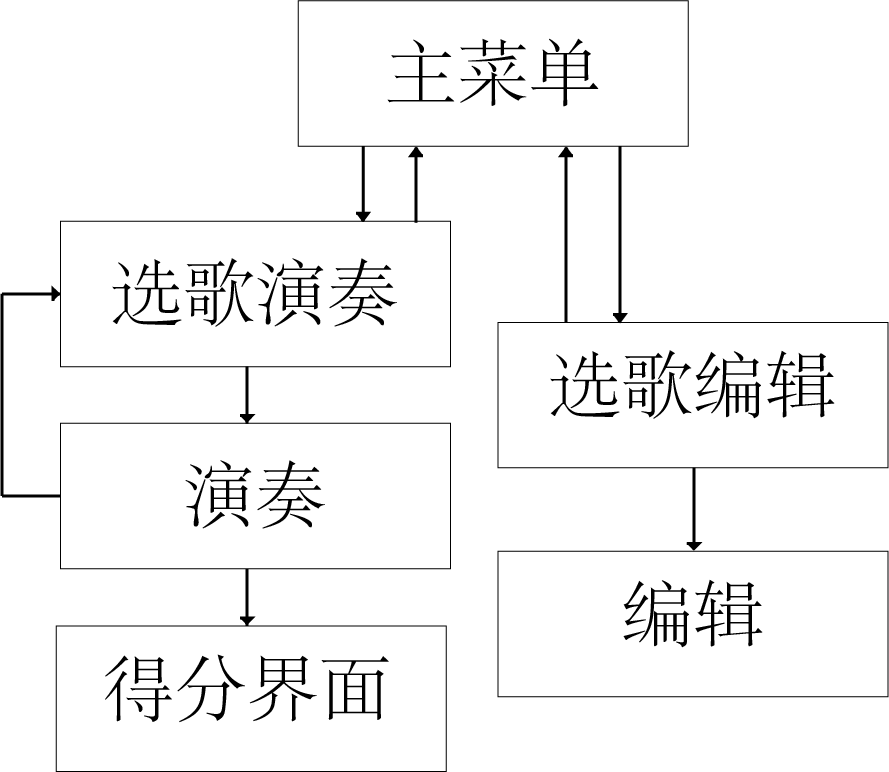
\includegraphics[width=20em]{progress.png}\\
  \caption{}\label{}
\end{figure}
\paragraph{}
游戏内有五个界面,按照图中流程可以互相转换。\\
\textbf{主菜单}
\begin{figure}[H]
  \centering
  % Requires \usepackage{graphicx}
  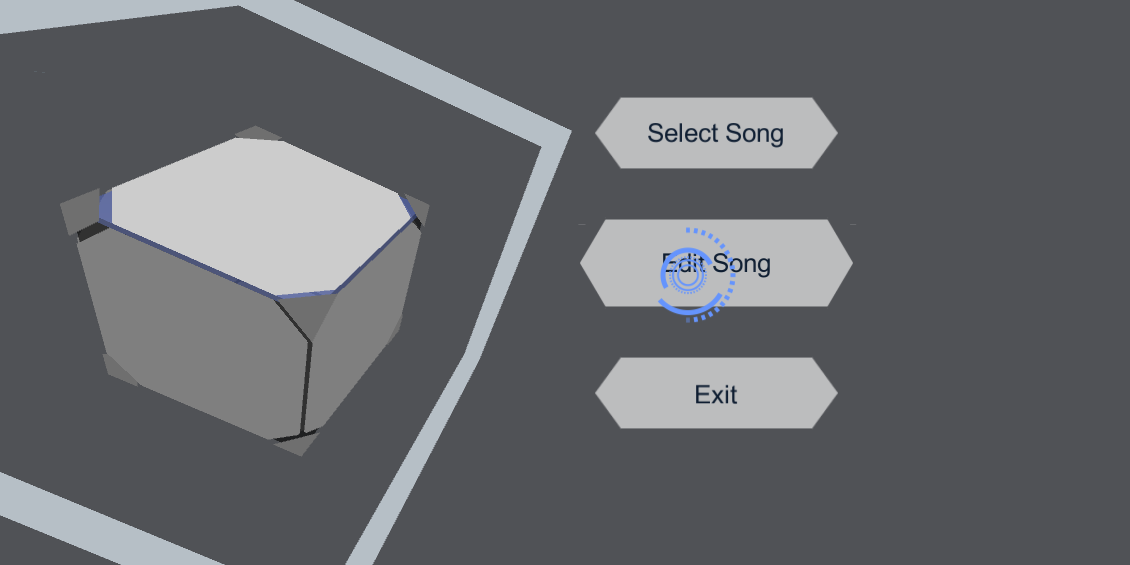
\includegraphics[width=28em]{mainMenu.png}\\
  \caption{}\label{}
\end{figure}
\newpage
\textbf{选歌}
\begin{figure}[H]
  \centering
  % Requires \usepackage{graphicx}
  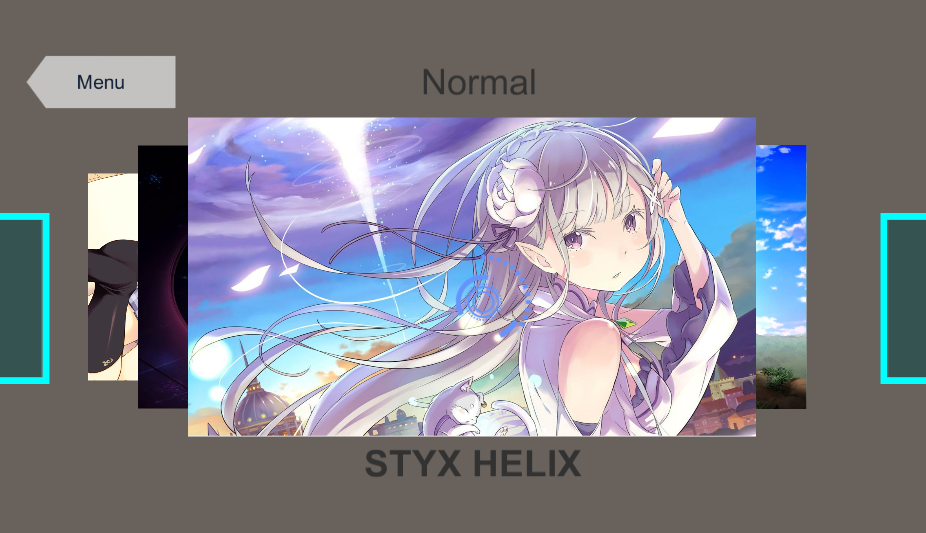
\includegraphics[width=28em]{selectMusic.png}\\
  \caption{}\label{}
\end{figure}
\textbf{编辑}
\begin{figure}[H]
  \centering
  % Requires \usepackage{graphicx}
  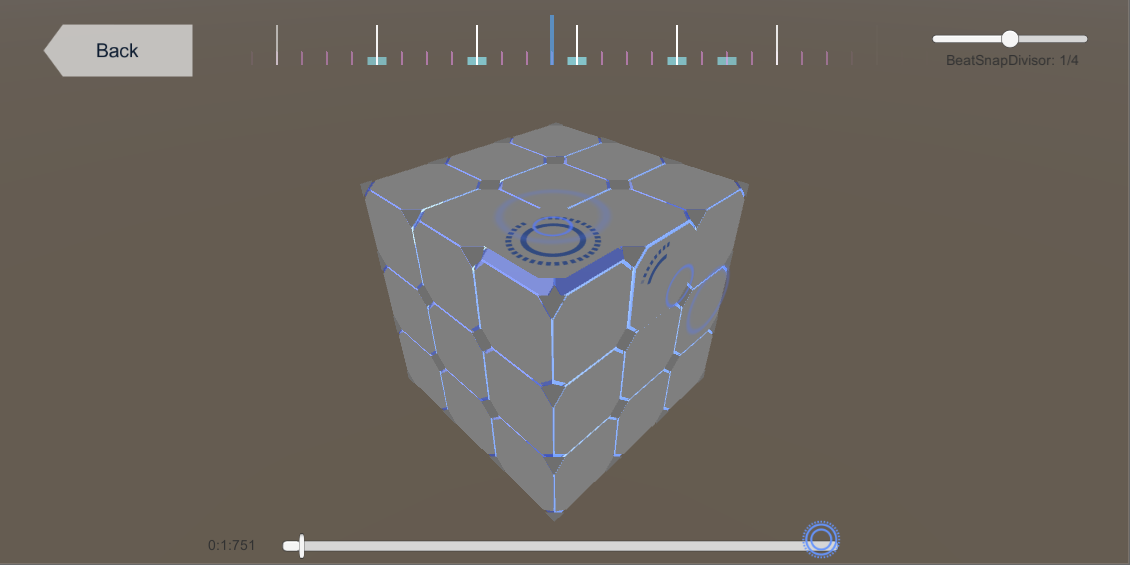
\includegraphics[width=28em]{edit.png}\\
  \caption{}\label{}
\end{figure}
\textbf{演奏}
\begin{figure}[H]
  % Requires \usepackage{graphicx}
  \begin{minipage}{0.5\linewidth}
    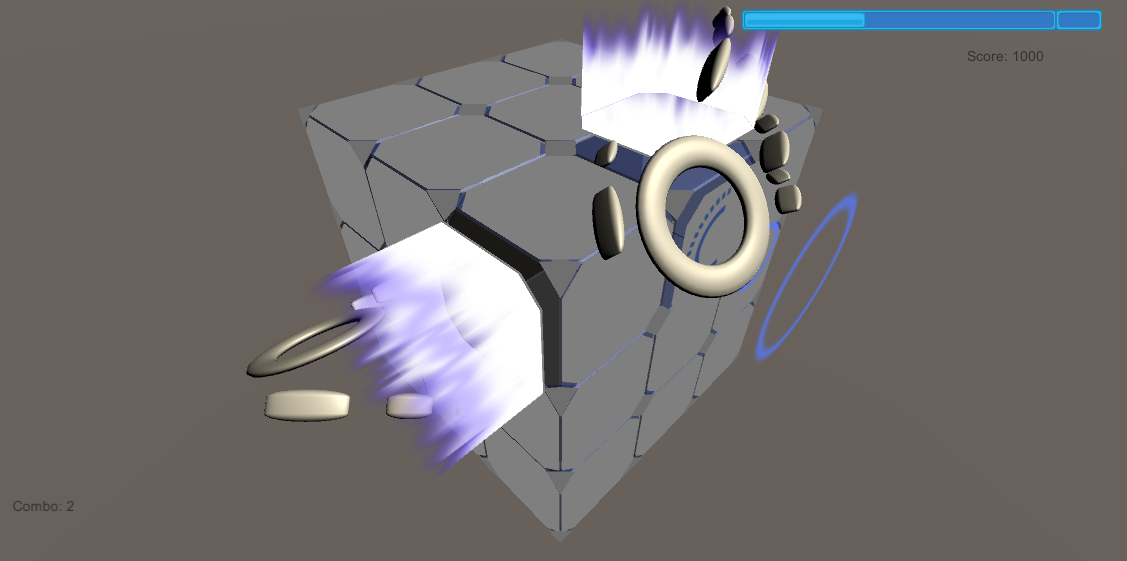
\includegraphics[width=15em]{inGame.png}\\
    \caption{}\label{}
  \end{minipage}
  \begin{minipage}{0.5\linewidth}
    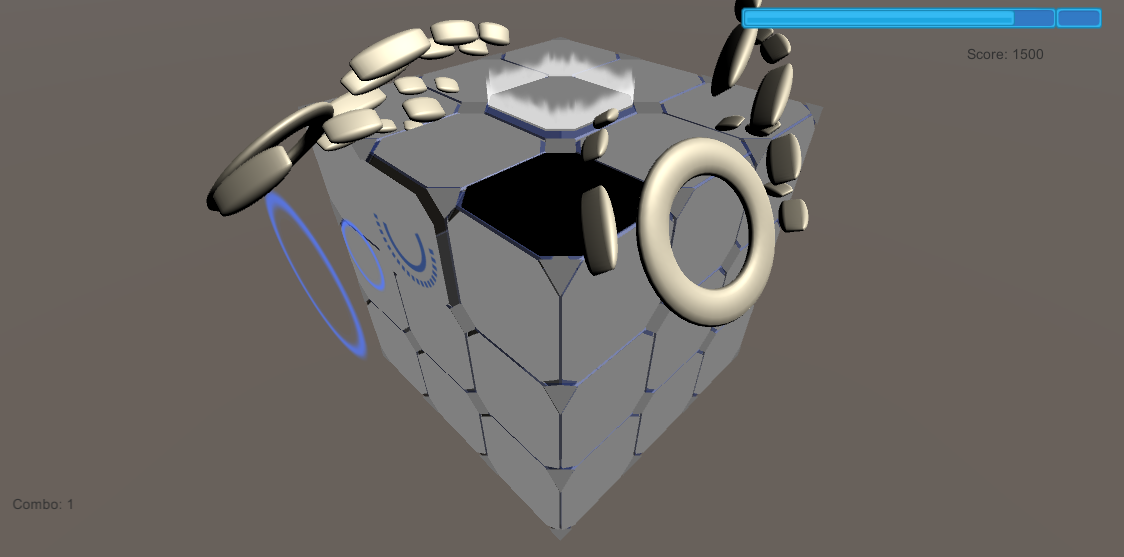
\includegraphics[width=15em]{inGame2.png}\\
    \caption{}\label{}
  \end{minipage}
\end{figure}
\paragraph{数据格式}
歌曲和图谱文件放在\textbf{Songs}文件夹内,每一个文件夹是一个单独的\textbf{Song},每一个\textbf{Song}文件夹内有一个\textbf{mci}文件和若干个\textbf{mcb}文件。其中\textbf{mci}文件记录了这首歌曲的一些信息,每个\textbf{mcb}文件则是一
个单独的难度,文件头部记录了此难度的信息,接下来是具体的物件信息。
\begin{figure}[H]
  \centering
  % Requires \usepackage{graphicx}
  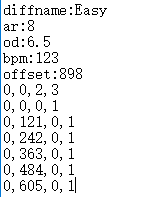
\includegraphics[width=8em]{mci.png}\\
  \caption{}\label{}
\end{figure}
\paragraph{}
数据部分有多行四列,每一行是一个单独的物件,对应着游戏内的一次需要用户操作的
音符。而四列从左到右分别为:物件类型编号、时间戳(毫秒)、方块或层数编号、方
向编号
\subsection{实现方法}
\subsection{制作难点}
\paragraph{Unity3D内置音频支持问题}
由于希望能够用户自制图谱,所以游戏需要从外部读取文件(包括音频文件)。但是经
过查询文档和测试发现,Unity3D内置的音频支持在Windows平台下,只能从外部读取
\textbf{.ogg}格式的文件。
\paragraph{解决方案}
一般使用C\#进行音频读取或处理时都采用\textbf{NAudio}库,但是Unity3D支持的
\textbf{\.net}框架与\textbf{NAudio}不兼容。我们使用了一个第三方修改后重新编
译的\textbf{NAudio}的\.dll文件并自己实现了一个使用\textbf{NAudio}接口的音频
读取器\textbf{AudioLoader}
\paragraph{}
现阶段采用的方式是只支持\textbf{.ogg}格式的音频,以后准备使用\textbf{NAudio}库来支持大部分格式的音频文件,并将数据加载进Unity3D内置的音频支持类中。
\paragraph{界面美观和游戏画面}
界面和游戏画面一直是我们头疼的问题,因为没有相关专业的同学帮助,我们花费了不
少精力在做动画和美化UI上。
\paragraph{LeapMotion与UI的交互}
由于LeapMotion的API特性,不易使用Unity3D原生UI,我们根据自己的需求重新编写了
一套UI交互的脚本。交互有两种方法:
\begin{itemize}
  \item 将手指位置映射到Canvas上,代替鼠标与其他原生UI交互,并且可以通过手
      势检测完成“点击按钮”的操作
  \item 使用实体作为UI,根据碰撞检测实现交互
\end{itemize}
\paragraph{LeapMotion精度问题}
虽然LeapMotion一直吹捧自己的高精度、低延迟,在经过它的驱动Orion升级后,
LeapMotion的性能得到了长足的提升。
\begin{description}
  \item[精度] 虽然精度有待提高,但是对于一个3X3一共27个面的魔方来说,能够在4立方英尺工作的LeapMotion基本足够了
  \item[延迟] 一般音乐游戏的最佳判定在正负20到30毫秒左右,而要使玩家获取较
      为舒服的游戏体验,游戏帧数可能需要达到240或更高。由于不易测量,我们
      使用官方提供的参数——最大290帧,也基本满足我们的需求。
\end{description}
\paragraph{}
但是在实际测试中,我们发现LeapMotion有不少问题:
\begin{enumerate}
  \item 误识别(如将脸识别为手,中指识别为食指)
  \item 无法识别
  \item 识别固定关节时会将抖动幅度放大
\end{enumerate}
\section{项目完成度}
\subsection{已实现功能}
\paragraph{}
我们通过一个学期的努力,完成了一个可以通过LeapMotion控制游玩和制作图谱的音乐
游戏。
\paragraph{代码}
项目为Unity3D工程,主要资源和代码在项目目录的Assets文件夹下,在Assets文件夹
下:
\begin{description}
  \item[Scenes] 所有游戏场景的场景文件和控制代码
  \item[Plugins] 第三方动态链接库
  \item[UI] UI控件、动画和控制脚本
  \item[LeapMotion、LeapMotionVR] LeapMotion及其扩展库
  \item[MusiCube] 方块弹出、击打以及旋转动画
  \item[Resources] UI的动画资源文件
  \item[StreamingAssets] 歌曲存放
\end{description}
\newpage
实现了游戏中“魔方”类\textbf{MagiCube}的大部分逻辑控制代码,并完成了一个控制它的编辑器类\textbf{MapMaker}以及游戏控制类\textbf{GameManager}。通过这两个类基本可以实现游戏和编辑的两种主要功能。\\
现阶段完成了\textbf{MagiCube}的方块弹出动画和玩家触碰的反馈动画和控制。\\
同时们还完成了游戏主界面——选歌界面、主菜单和得分界面,并进行了美化。
\begin{figure}[H]
  \centering
  % Requires \usepackage{graphicx}
  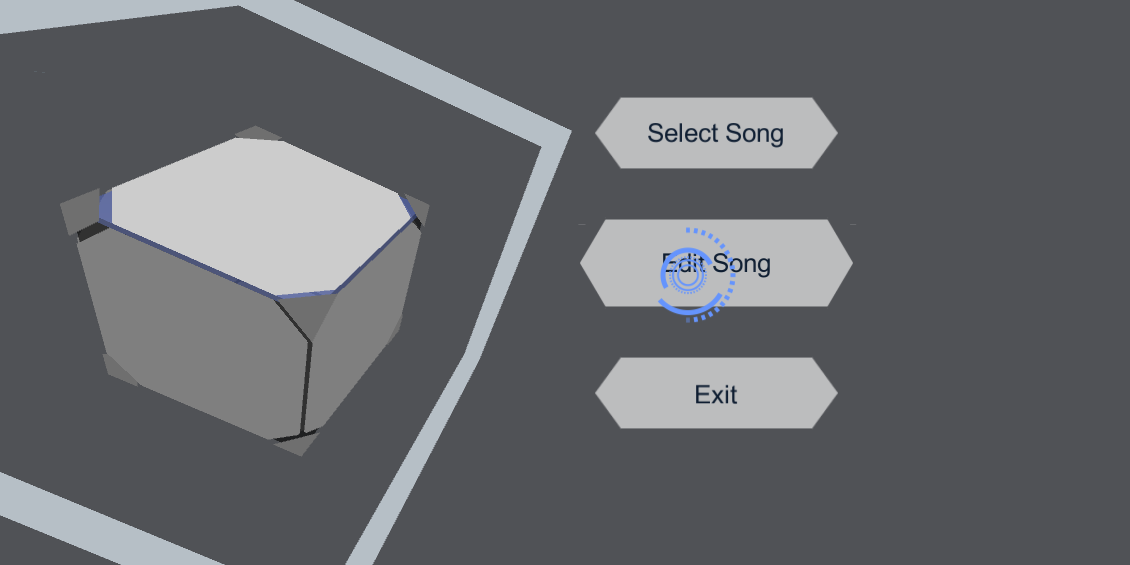
\includegraphics[width=40em]{mainMenu.png}\\
  \caption{}\label{}
\end{figure}
\paragraph{模型/动画}
完成了“魔方”的模型和动画制作,动画包括
\begin{enumerate}
  \item 编辑时选择
  \item 编辑时取消选择
  \item 游戏时弹出
  \item 游戏时击打 - Perfect判定
  \item 游戏时击打 - Good判定
  \item 游戏时击打 - Normal判定
  \item 游戏时击打 - Miss判定
\end{enumerate}
\paragraph{}
动画的实现是通过代码和动画曲线实现的,可以在Unity3D内灵活调整动画参数,在编辑器和游戏运行时都可以改变动画效果,并提供了单帧播放的接口。
\begin{figure}[H]
  \centering
  % Requires \usepackage{graphicx}
  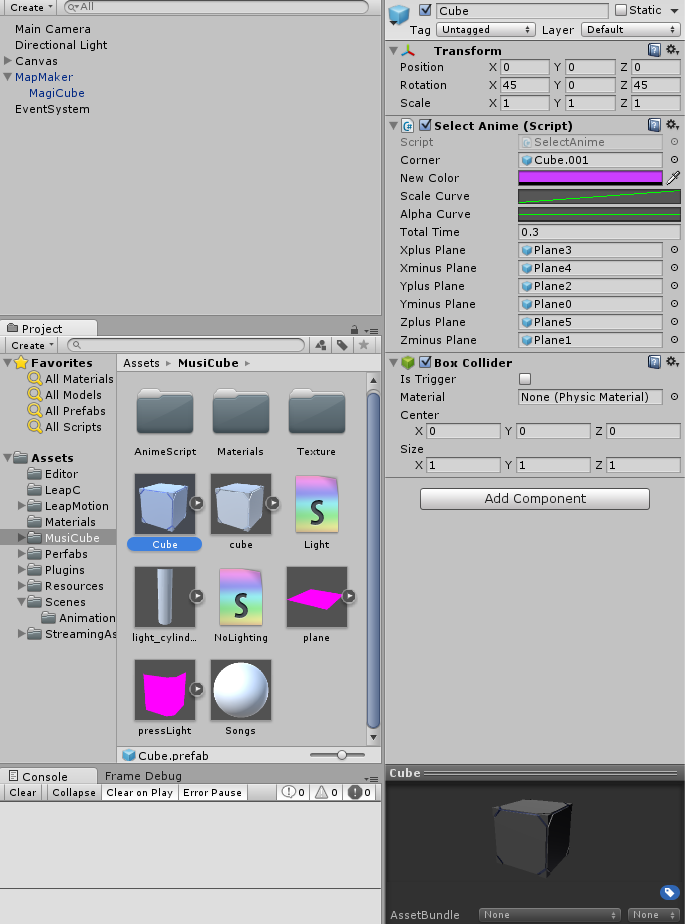
\includegraphics[width=18em]{work1.png}\\
  \caption{}\label{}
\end{figure}
\newpage
\subsection{未来展望}
在一个学期的努力下,我们已经实现了一个基础的能够配合音乐节拍游玩的游戏。对于
Musicube,我们仍有一下的展望
\begin{enumerate}
  \item 完成游戏内旋转的判定
  \item 提供更多游戏方式
  \item 增加拖动音频文件开始编辑的功能
  \item 打包歌曲及铺面功能
  \item 构建玩家社区,实现上传图谱、共享图谱等功能
  \item 进一步美化UI
\end{enumerate}
\end{document}
